\chapter{State of Art}%
\label{chap-state}

Systematic literature review (SRL) studies are traditionally in software engineering, and software refactoring brings an excellent background for study analysis and classifications. As time passes, studies become obsolete as new articles are published monthly. A forward snowballing was proposed to update the systematic literature reviews on software refactoring.

This chapter presents the results of snowballing carried out to to ensure that there is no other tool like RMT. This chapter is structured as \Cref{sec-background} describing the research methodology; \Cref{sec-methods} explaining the methods chosen to apply to the research; \Cref{sec-results} showing the results obtained in the study; \cref{sec-trends} explaining the trends in the research; \Cref{sec-cloasing-remarks} are the closing remarks.

\section{Background}
\label{sec-background}
According to \cite{bernard2006}, the snowballing technique is a non-probabilistic sampling technique that allows the reach of hard-to-reach or little-known populations. It occurs due to its mechanism of establishing a network of relationships among the elements, creating a chain of references.

The technique has three objectives: to improve the understanding of a theme, verify the possibility of conducting a more extensive study, and develop methods to be employed in subsequent studies and phases \cite{vinuto2014}. Snowballing is used mainly for experimental purposes.

The procedure for following the Snowballing technique is described in the following steps: start set, iterations (backward snowballing, forward snowballing, and inclusion and exclusion), identification of the authors, and data extraction \cite{Wohlin2014}.

The first step of snowballing is creating a starting set of papers; a viable option is to use search engines such as Google Scholar. It is an excellent alternative to avoid bias in favor of any author \cite{Wohlin2014}.

\textcite{Kitchenham2013} chose a set of works to start the snowballing; they preferred to use two conference proceedings, the Evaluation and Assessment in Software Engineering and Empirical Software Engineering and Measurement Searching, from 2005 to mid-2012. We chose first to utilize a database search with a string and search engines as it avoids the bias of a starter set of SRL before the forward snowballing to update the fancied SLR.

The title and abstract are the elements to consider when selecting suitable candidate papers. The main goal is to avoid unrelated works, but only if they are explicitly irrelevant, and the premise is to include any paper that may be relevant. To select or remove articles, all authors must agree, and if there is any estrangement, discussions may occur until their consent is defined \textcite{Kitchenham2013}.

After establishing the initial set, the iteration step is performed by performing Backward Snowballing and Forward Snowballing, including and excluding new jobs in the collection \cite{Wohlin2014}.

Backward snowballing consists of using the list of references to identify new articles to be analyzed later on. The first step is to review the references and discard the papers that do not meet the essential research criteria. The second step is to remove the reports that have already been examined from the list. The first two steps are about extracting information from the article, and a new article should not be studied if there is not enough information in the analyzed document \cite{Wohlin2014}.

Conversely, forward snowballing consists of using the list of citations to identify new articles to be analyzed later. The first step is to review the citations in an online database and discard papers that do not meet the essential criteria. The following steps follow the same concept as forward-backward snowballing \cite{Felizardo2016}.

\section{Methods}
\label{sec-methods}
Database searches were used to start a systematic literature review update. For instance, to find a search string, the databases were chosen to search for and determine the exclusion and inclusion to decide which of the found studies are adequate to enter as a starter set for the forward snowballing.

It is challenging to assemble a suitable string, as the terminology used in software engineering is not standardized. Using a specific keyword may find a few relevant articles and even miss some suitable works; otherwise, using generic keywords may result in irrelevant articles, creating unnecessary labor \cite{Wohlin2014}.

To find the starter set of SLR to apply the forward snowballing, a database search with a specific set of keywords was determined, and the found collection of papers will be updated as a result of the process. The search string to initiate the snowballing approach is (("systematic literature review") OR ("systematic review") OR ("systematic mapping review") OR ("systematic mapping") ) AND "software refactoring" and includes all the main desired topics to search. An inclusion and exclusion criteria list was defined to select the papers returned by the search string. The inclusion criteria are as follows:

\begin{itemize}
    \item The publishing year of the articles must be between 1992 and 2022, as \textcite{Opdyke1992} was the first person to publish with the refactoring term;
    \item Systematic literature review articles and systematic mapping reviews about software refactoring methods, frameworks, technics; or applications or development, methods or practices code smells detections;
\end{itemize}

The criteria for exclusions are as follows.

\begin{itemize}
    \item Article not written in English or Portuguese;
    \item Non-source code studies or architecture refactoring;
    \item Abstract, posters, patents, and keynotes;
\end{itemize}

The standards must be followed by reading the article's title to filter the studies using the above criteria. If it already has the information to be accepted, no more reading is necessary for inclusion; if only the title is insufficient, the abstract is thoroughly read to understand more about the paper's objectives. The whole article is read if there is still doubt about the exclusion or inclusion. \textcite{Wohlin2014} does not recommend reading the report from the beginning; instead, he argues that it is best to read the most relevant parts to make a decision.
The search engines were Google Scholar, Springer, Science Direct, ResearchGate, IEEE Xplore, and ACM. From these bases, 804 articles were divided per database: 689 from Google Scholar, 43 from Springer, 32 from Science Direct, 25 from ResearchGate, 12 from ACM, and three from IEEE Xplore, as shown in \Cref{tab-reviews}.

To apply forward snowballing, Google Scholar was chosen to look for citations, as it is an excellent way to avoid bias \cite{Wohlin2014}. All articles were subjected to one interaction with the original SRL as sed \textcolor{red}{o que seria sed?} set, evidenced by \textcite{Wohlin2020} as the most cost-effective approach to update the studies. The diagram in \Cref{fig-snow} exemplifies the whole search method. 

\begin{figure}[ht!]
\SetCaptionWidth{\textwidth}
\caption{Search Method Diagram}
\label{fig-snow}
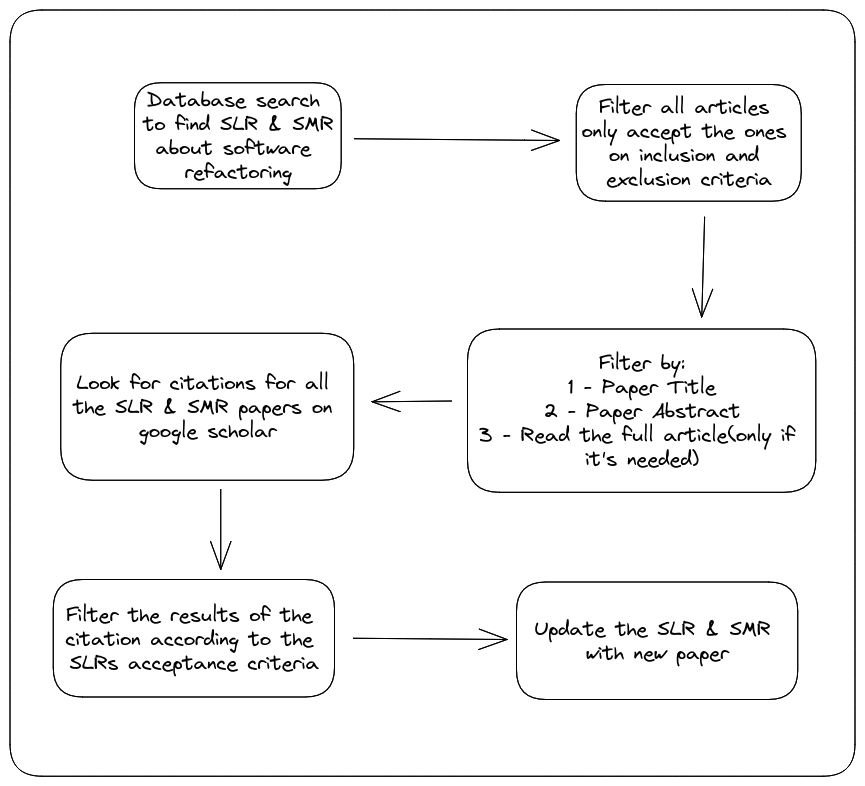
\includegraphics[width =100mm]{Chapter-3/Figures/snowballing_diagram.png}
\SourceOrNote{Own authorship (2023)}
\end{figure}
\FloatBarrier

As in the database search, snowballing inclusion and exclusion criteria must be applied in the papers that have cited the current SRL. The requirements must come from the starting set of documents \cite{Wohlin2020}. Reading every SRL, it generally finds a section explaining those accepted standards.


\section{Results}
\label{sec-results}
\Cref{tab-reviews} shows all the papers found on the database search to achieve the start set for snowballing; it contains an id composed of S representing the start and a number. The table is sorted by title and contains the total number of citations found in Google Scholar for each article and the reference.

\begin{tabframed}
\caption{Select papers from database search}
\label{tab-reviews}
\begin{tabularx}{\textwidth}{|e{}@{},{}@{}|p{9cm}|c|p{3cm}@{}|}
\toprule%
\multicolumn{1}{|@{}c|}{\textbf{Key}}        &
\multicolumn{1}{c|}{\textbf{Tile}}    &
\multicolumn{1}{c|}{\textbf{Citation  Nº}}  &
\multicolumn{1}{c@{}|}{\textbf{Ref}}        \\
\midrule% 
S1  & 30 Years of Software Refactoring Research:A Systematic Literature Review                           & 13          & \citeauthor*{Abid2020}                               \\
S2  & A Literature Review on Code Smells and Refactoring                                                 & 17          & \citeauthor*{Ruben2010}                              \\
S3  & A Systematic Literature Review on Software Refactoring                                             & 0           & \citeauthor*{Elhazzat2020}                           \\
S4  & A Systematic Literature Review on Software-refactoring Techniques, Challenges, and Practices       & 0           & \citeauthor*{Akhtar2022}                             \\
S5  & A systematic literature review: Refactoring for disclosing code smells in object oriented software & 74          & \citeauthor*{Singh2018b}                              \\
S6  & A systematic literature survey of software metrics, code smells and refactoring techniques         & 15          & \citeauthor*{Agnihotri2020}                          \\
S7  & A systematic mapping of literature on software refactoring tools                                   & 3           & \citeauthor*{Tavares2018}                            \\
S8  & A systematic review on search-based refactoring                                                    & 78          & \citeauthor*{Mariani2017}                            \\
S9  & Automatic software refactoring: a systematic literature review                                     & 40          & \citeauthor*{Baqais2020}                             \\
S10 & Classification and Summarization of Software Refactoring Researches: A Literature Review Approach  & 4           & \citeauthor*{Abebe2014b}                              \\
S11 & Code Smells and Refactoring: A Tertiary Systematic Review of Challenges and Observations           & 47          & \citeauthor*{Lacerda2020}                            \\
S12 & Multi-Objective Optimization Techniques for Software Refactoring: A Systematic Literature Review   & 1           & \citeauthor*{Rafique2019}                            \\
S13 & On preserving the behavior in software refactoring: A systematic mapping study                     & 15          & \citeauthor*{AlOmar2021}                             \\
S14 & Trends, opportunities and challenges of software refactoring: A systematic literature review       & 42          & \citeauthor*{Abebe2014a}                              \\
S15 & Why , How , and When Refactorings are ( NOT ) Applied : A Systematic Literature Review             & 0           & \citeauthor*{Buriakovskyi2018}                                \\
\bottomrule%
\end{tabularx}
\SourceOrNote{Own authorship (2023)}           
\end{tabframed}
\FloatBarrier

The most crucial part of updating the SRLs in the acceptance criteria is that their interpretation will decide if a cited paper has the qualities to be included in its update. Most studies have an explicit acceptance criterion besides S3, S7, S10, and S12. Although S12 has no detailed parameters, the questions are well-defined enough to use as a selection method for snowballing; unfortunately, the paper has no citations. For S10, the criteria to include in the update were the classification made from the SLR-selected articles. However, finding an alternative to filter the citations became less secure in fitting the original article because the author did not have a particular sentiment. \textcolor{red}{não compreendi a frase final}

Multiple articles did not include some styles of publications, such as abstracts, posters, and keynotes for S8, S9, and S13, gray literature for S1, S8, and S9, doctoral symposiums, books, and theses for S8 and S9. In the gray literature, it may not be the most reasonable guideline to follow because, as shown in articles S1 and S11, the first time worked with the term refactoring was in 1992 by \textcite{Opdyke1992}, which was a Ph.D. thesis. According to \textcite{Buriakovskyi2018}, only after the published book \textcite{fowler2018refactoring} did the active research on the practical use of refactoring begin. This would exclude both studies from S8 and S9.

The number of studies selected and filtered for each article was quite different; after removing duplicates, the final result was six articles for S1, 4 for S2, 13 for S5, 4 for S6, 16 for S8, 5 for S9, 1 for S10, 15 for S11, and 1 for S13. Sixty-five possible papers will be included in future SLR updates as the analyses cover each article's approval criteria.

 \Cref{tab-snow} shows all the selected papers from applying the forward snowballing and following the acceptance criterion from all the SLRs. The first row has the ID studies from the starter set referenced; the cited papers ID is in n the second column referenced with the SLR ID and a capital C and a number; the title is in the third column, and the bibliographic reference is in the last column.

\begin{longtable}{|e{}@{},{}@{}|c|p{9cm}|p{3cm}@{}|}
%% Cabeçalho da primeira página
\caption{Resultant Articles with design patterns methods}
\label{tab-snow}                                              \\[\belowcaptionskip]
\multicolumn{4}{@{}r@{}}{\textbf{(continue)}}                 \\[\belowcaptionskip]
\toprule%
\multicolumn{1}{|@{}c|}{\textbf{Key}}        &
\multicolumn{1}{c|}{\textbf{Id}}            &
\multicolumn{1}{c|}{\textbf{Title}}         &
\multicolumn{1}{c@{}|}{\textbf{Ref}}        \\
\midrule%
\endfirsthead%
%% Cabeçalho das páginas (exceto primeira e última)
\caption[]{Resultant Articles with design patterns methods}   \\[\belowcaptionskip]
\multicolumn{4}{@{}r@{}}{\textbf{(continuation)}}             \\[\belowcaptionskip]
\toprule%
\multicolumn{1}{|@{}c|}{\textbf{Key}}        &
\multicolumn{1}{c|}{\textbf{Id}}            &
\multicolumn{1}{c|}{\textbf{Title}}         &
\multicolumn{1}{c@{}|}{\textbf{Ref}}        \\
\midrule%
\endhead%
%% Cabeçalho da última página
\caption[]{Resultant Articles with design patterns methods}   \\[\belowcaptionskip]
\multicolumn{4}{@{}r@{}}{\textbf{(conclusion)}}               \\[\belowcaptionskip]
\toprule%
\multicolumn{1}{|@{}c|}{\textbf{Key}}        &
\multicolumn{1}{c|}{\textbf{Id}}            &
\multicolumn{1}{c|}{\textbf{Title}}         &
\multicolumn{1}{c@{}|}{\textbf{Ref}}        \\
\midrule%
\endlasthead%
%% Rodapé da última página
\bottomrule%
\LTSourceOrNote{Own authorship (2023)}           \\
\endlastfoot% 

S1  &        &                                                                                                                                                                                                                                               &                                 \\
    & S1-C1   & Generation of refactoring algorithms by grammatical evolution                                                                                                                                                                                  & \citeauthor*{Mariani2022}     \\
    & S1-C2   & Refactorings and Technical Debt in Docker Projects: An Empirical Study                                                                                                                                                                         & \citeauthor*{Ksontini2021}    \\
    & S1-C3   & RefDetect: A Multi-Language Refactoring Detection Tool Based on String Alignment                                                                                                                                                               & \citeauthor*{Moghadam2021}    \\
    & S1-C4   & Supporting refactoring of BDD specifications—An empirical study                                                                                                                                                                                & \citeauthor*{Irshad2022}      \\
    & S1-C5   & Refactoring Techniques for Improving Software Quality: Practitioners’ Perspectives                                                                                                                                                             & \citeauthor*{Ksontini2021}    \\
    & S1-C6   & Automated refactoring of legacy JavaScript code to ES6 modules                                                                                                                                                                                 & \citeauthor*{Paltoglou2021}   \\
S2  &        &                                                                                                                                                                                                                                               &                                 \\
    & S2-C1   & Design and Implementation of a Web-Based Application for Code Smells Repository                                                                                                                                                                & \citeauthor*{Bamizadeh2021}   \\
    & S2-C2   & Object-Oriented Code Metric-Based Refactoring Opportunities Identification Approaches: Analysis                                                                                                                                                & \citeauthor*{Bassey2017}      \\
    & S2-C3   & Analysing The Effects Of Refactoring On Software Quality Attributes                                                                                                                                                                            & \citeauthor*{Singh2018a}       \\
    & S2-C4   & Measuring Code Smells and Anti-Patterns                                                                                                                                                                                                        & \citeauthor*{Reeshti2019}     \\
S5  &        &                                                                                                                                                                                                                                               &                                 \\
    & S5-C1   & Code Smell Refactoring for Energy Optimization of Android Apps                                                                                                                                                                                 & \citeauthor*{Reeshti2021}     \\
    & S5-C2   & Software Engineering Paradigm for Real-Time Accurate Decision Making for Code Smell Prioritization                                                                                                                                             & \citeauthor*{Singh2021}       \\
    & S5-C3   & A Framework to Improve Quality of a Java System by Performing Refactoring                                                                                                                                                                      & \citeauthor*{singhAndBindal2020}       \\
    & S5-C4   & Detecting Sudden Variations in Web Apps Code Smells’ Density: A Longitudinal Study                                                                                                                                                             & \citeauthor*{Rio2021}         \\
    & S5-C5   & Controlling software evolution process using code smell visualization                                                                                                                                                                          & \citeauthor*{Nabilah2019}     \\
    & S5-C6   & PHP code smells in web apps: survival and anomalies                                                                                                                                                                                            & \citeauthor*{Rio2021}         \\
    & S5-C7   & Bad Smell Detection Using Machine Learning Techniques: A Systematic Literature Review                                                                                                                                                          & \citeauthor*{Al-Shaaby2020}   \\
    & S5-C8   & Recovering Android Bad Smells from Android Applications                                                                                                                                                                                        & \citeauthor*{Rasool2020}      \\
    & S5-C9   & To improve code structure by identifying move method opportunities using frequent usage patterns in source-code                                                                                                                                & \citeauthor*{Singh2019}       \\
    & S5-C10  & Using software metrics to detect temporary field code smell                                                                                                                                                                                    & \citeauthor*{Gupta2020a}      \\
    & S5-C11  & Rank-based univariate feature selection methods on machine learning classifiers for code smell detection                                                                                                                                       & \citeauthor*{Jain2022}        \\
    & S5-C12  & TFfinder: A Software tool to discover Temporary Field code smell                                                                                                                                                                               & \citeauthor*{Gupta2020b}      \\
    & S5-C13  & Analysis of code smell to quantify the refactoring                                                                                                                                                                                             & \citeauthor*{Sehgal2017}      \\
S6  &        &                                                                                                                                                                                                                                               &                                 \\
    & S6-C1   & Does Code Complexity Affect the Quality of Real-Time Projects?: Detection of Code Smell on Software Projects using Machine Learning Algorithms                                                                                                 & \citeauthor*{Patnaik2021b}    \\
    & S6-C2   & A hybrid approach to identify code smell using machine learning algorithms                                                                                                                                                                     & \citeauthor*{Patnaik2021a}     \\
    & S6-C3   & Illustration and detection of exception handling bad smells                                                                                                                                                                                    & \citeauthor*{Tarwani2021}     \\
    & S6-C4   & Automated refactoring of legacy JavaScript code to ES6 modules                                                                                                                                                                                 & \citeauthor*{Paltoglou2021}   \\
S8  &        &                                                                                                                                                                                                                                               &                                 \\
    & S8-C1   & Enabling Decision and Objective Space Exploration for Interactive Multi-Objective Refactoring                                                                                                                                                  & \citeauthor*{Rebai2020}       \\
    & S8-C2   & Explainable Search-Based Refactoring                                                                                                                                                                                                           & \citeauthor*{Abid2021c}       \\
    & S8-C3   & Intelligent Change Operators for Multi-Objective Refactoring                                                                                                                                                                                   & \citeauthor*{Abid2021a}       \\
    & S8-C4   & Interactive Decision and Objective Space Exploration for Search Based Refactoring                                                                                                                                                              & \citeauthor*{Rebai2019}       \\
    & S8-C5   & A Many-Objective Estimation Distributed Algorithm Applied to Search Based Software Refactoring                                                                                                                                                 & \citeauthor*{Botelho2018}     \\
    & S8-C6   & X-SBR: On the Use of the History of Refactorings for Explainable Search-Based Refactoring and Intelligent Change Operators                                                                                                                     & \citeauthor*{Abid2021b}       \\
    & S8-C7   & The Effectiveness of Supervised Machine Learning Algorithms in Predicting Software Refactoring                                                                                                                                                 & \citeauthor*{Aniche2022}      \\
    & S8-C8   & Improving Readability of Scratch Programs with Search-based Refactoring                                                                                                                                                                        & \citeauthor*{Adler2021}       \\
    & S8-C9   & Untangling the Knot: Enabling Architecture Evolution with Search-Based Refactoring                                                                                                                                                             & \citeauthor*{Ivers2022}       \\
    & S8-C10  & Harnessing deep learning algorithms to predict software refactoring                                                                                                                                                                            & \citeauthor*{Alenezi2020}     \\
    & S8-C11  & DEPICTER: A Design-Principle Guided and Heuristic-Rule Constrained Software Refactoring Approach                                                                                                                                               & \citeauthor*{Zhao2022}        \\
    & S8-C12  & EASIER: An Evolutionary Approach for Multi-objective Software ArchItecturE Refactoring                                                                                                                                                         & \citeauthor*{Arcelli2018}     \\
    & S8-C13  & Unsupervised Learning For Refactoring Pattern Detection                                                                                                                                                                                        & \citeauthor*{Farah2021}       \\
    & S8-C14  & Model refactoring by example: A multi-objective search based software engineering approach                                                                                                                                                     & \citeauthor*{Ghannem2018}     \\
    & S8-C15  & A survey of many-objective optimisation in search-based software engineering                                                                                                                                                                   & \citeauthor*{Ramirez2019}     \\
    & S8-C16  & Applying design patterns in the search-based optimization of software product line architectures                                                                                                                                               & \citeauthor*{Guizzo2019}      \\
S9  &        &                                                                                                                                                                                                                                               &                                 \\
    & S9-C1   & An automated extract method refactoring approach to correct the long method code smell                                                                                                                                                         & \citeauthor*{Shahidi2022}     \\
    & S9-C2   & Automated Refactoring of Unbounded Queries in Software Automation Platforms                                                                                                                                                                    & \citeauthor*{Fernandes2021}   \\
    & S9-C3   & Cross-Project Software Refactoring Prediction Using Optimized Deep Learning Neural Network With the Aid of Attribute Selection                                                                                                                 & \citeauthor*{Panighrahi2022}  \\
    & S9-C4   & An automatic refactoring framework for replacing test-production inheritance by mocking mechanism                                                                                                                                              & \citeauthor*{Wang2021}        \\
    & S9-C5   & Refactoring Legacy Software for Layer Separation                                                                                                                                                                                               & \citeauthor*{Khalilipour2021} \\
S10 &        &                                                                                                                                                                                                                                               &                                 \\
    & S10-C1  & Composite Refactoring: Representations, Characteristics and Effects on Software Projects                                                                                                                                                       & \citeauthor*{Bibiano2022}     \\
S11 &        &                                                                                                                                                                                                                                               &                                 \\
    & S11-C1  & RefDiff4Go: Detecting Refactorings in Go                                                                                                                                                                                                       & \citeauthor*{Brito2020}       \\
    & S11-C2  & Test smell detection tools: A systematic mapping study                                                                                                                                                                                         & \citeauthor*{Aljedaani2021}   \\
    & S11-C3  & An automated extract method refactoring approach to correct the long method code smell                                                                                                                                                         & \citeauthor*{Shahidi2022}     \\
    & S11-C4  & Automated refactoring of legacy JavaScript code to ES6 modules                                                                                                                                                                                 & \citeauthor*{Paltoglou2021}   \\
    & S11-C5  & Automatic detection of Long Method and God Class code smells through neural source code embeddings                                                                                                                                             & \citeauthor*{Kovačević2022}   \\
    & S11-C6  & Are Code Smell Co-occurrences Harmful to Internal Quality Attributes?: A Mixed-Method Study                                                                                                                                                    & \citeauthor*{Martins2020}     \\
    & S11-C7  & How do Code Smell Co-occurrences Removal Impact Internal Quality Attributes? A Developers' Perspective                                                                                                                                         & \citeauthor*{Martins2021}     \\
    & S11-C8  & "Project smells" -- Experiences in Analysing the Software Quality of ML Projects with mllint                                                                                                                                                   & \citeauthor*{van2022}         \\
    & S11-C9  & Toward the automatic classification of Self-Affirmed Refactoring                                                                                                                                                                               & \citeauthor*{AlOmar2021b}     \\
    & S11-C10 & A framework to improve quality of a Java system by performing refactoring Currently I am working on Disaster Management and energy efficient deployment View project A framework to improve quality of a Java system by performing refactoring & \citeauthor*{Singh2020}       \\
    & S11-C11 & TERTIARY STUDY on LANDSCAPING the REVIEW in CODE SMELLS                                                                                                                                                                                        & \citeauthor*{Yaqoob2021}      \\
    & S11-C12 & MARS: Detecting brain class/method code smell based on metric–attention mechanism and residual network                                                                                                                                         & \citeauthor*{Zhang2021a}       \\
    & S11-C13 & RAID: Tool Support for Refactoring-Aware Code Reviews                                                                                                                                                                                          & \citeauthor*{Brito2021}       \\
    & S11-C14 & Code smells detection and visualization: A systematic literature review                                                                                                                                                                        & \citeauthor*{Pereira2022}     \\
S13 &        &                                                                                                                                                                                                                                               &                                 \\
    & S13-C1  & Consistency validation method for Java fine-grained lock refactoring                                                                                                                                                                           & \citeauthor*{Zhang2021b}         
\end{longtable}
\FloatBarrier

It was possible to analyze that some papers cited more than one SLR with slightly different subjects but the same refactoring matter. The article by \textcite{Paltoglou2021} focuses on proposing refactoring legacy Javascript to a newer version called ES6 with many more features and reliability. The study appears on S1, S6, and S11.


\section{Trends}
\label{sec-trends}
This study used forward snowballing to propose a set of papers to be candidates for its original SRLs and SMRs.
A total of 65 papers could be included in their respective SRLs as the final step of the snowballing, considering the acceptance criteria of the original papers, which strictly ensures quality. In conclusion, snowballing showed an excellent and fast way to update an SRL and SMR.
The paper also shows how SLRs can age pretty well, like S9, a work from 2020 that already has 40 citations, where, after filtering, five possible studies were achieved to include in an update of this paper.

\textcolor{red}{acho que poderia ter outras conclusões. Achei o parágrafo seguinte repetitive. Precisa realmente dele?}

As argued, SRLs age quite rapidly; the same will happen with work as new papers are published every month, and some of those are likely to cite an article from the starter set, assuming that to avoid paper aging, they ought to apply an update of the database search and snowballing in a fixed data frame.

\section{Closing Remarks}
\label{sec-cloasing-remarks}

The main application of snowballing in this work is to find new methods to find opportunities to refactor Java code to apply design patterns by finding all refactoring-related SLRs and SMRs and applying the snowballing techniques. 

After the snowballing process, no new article was found on the desired topic. That shows the importance of RMT and how a tool that can integrate all refactoring methods to design patterns has not yet been found in the academy and can change how developers apply refactorings to their projects.